\documentclass[twoside,11pt]{article}


% Any additional packages needed should be included after jmlr2e.
% Note that jmlr2e.sty includes epsfig, amssymb, natbib and graphicx,
% and defines many common macros, such as 'proof' and 'example'.
%
% It also sets the bibliographystyle to plainnat; for more information on
% natbib citation styles, see the natbib documentation, a copy of which
% is archived at http://www.jmlr.org/format/natbib.pdf

% Available options for package jmlr2e are:
%
%   - abbrvbib : use abbrvnat for the bibliography style
%   - nohyperref : do not load the hyperref package
%   - preprint : remove JMLR specific information from the template,
%         useful for example for posting to preprint servers.
%fhajkfhcuhfkahficdaui
% Example of using the package with custom options:
%
% \usepackage[abbrvbib, preprint]{jmlr2e}

\usepackage[preprint]{jmlr2e}
\usepackage{array}
\usepackage{longtable}
\usepackage{booktabs}
\usepackage{amsmath}
\usepackage{amssymb}

\ShortHeadings{Novel Approach to deal with Data Imbalance in Automobile Insurance Fraud Data}{Alshamsi, Farhan and Mohammed}
\firstpageno{1}

\begin{document}

\title{Novel Approach to deal with Data Imbalance in Automobile Insurance Fraud Data}

\author{\name Abdus Saboor Gaffari Mohammed \email b00105302@aus.edu \\
        \addr Department of Computer Science \& Engineering\\
        Master of Science in Machine Learning\\
        American University of Sharjah\\
        Sharjah, UAE
        \AND
        \name Alizar Farhan \email b00106512@aus.edu \\
        \addr Department of Computer Science \& Engineering\\
        Master of Science in Computer Engineering\\
        American University of Sharjah\\
        Sharjah, UAE
        \AND
        \name Khalifa Alshamsi \email b00078654@aus.edu \\
        \addr Department of Computer Science \& Engineering\\
        Master of Science in Machine Learning\\
        American University of Sharjah\\
        Sharjah, UAE
       } 

\maketitle

\begin{abstract}%   <- trailing '%' for backward compatibility of .sty file

Our research addresses the critical issue of detecting automotive insurance fraud, a global problem that results in significant financial losses to the insurance companies and higher premium costs to policyholders. Auto-mobile insurance claim data suffers from data imbalance as there are less number of fraudulent insurance claims when compared to non-fraudulent claims. When we evaluated the generated datasets with machine learning models such as XGBoost and Random Forest, as well as classic resampling approaches, we got significant results in fraud detection accuracy, precision-recall and F1-score, even with imbalanced data available on the internet. This study encourages  the potential of merging generative models and advanced classifier, laying a solid foundation for fraud detection systems in the industry and opening the way for future advances in hyper-parameters tuning and ensemble learning in study Machine Learning and models.

\end{abstract}

\begin{keywords}
TVAE, Machine Learning, Automobile Insurance Fraud Detection, insurance fraud, data imbalance, synthetic data, SMOTE, XGBoost, Random Forest
\end{keywords}



\section{Introduction} 
The insurance sector is one of the oldest and largest financial sectors, providing financial protection from losses to individuals. Insurance is an agreement between an insurer and insured party (policyholder), in which the insurer promises financial compensation to the insured party in cases of an accident or specific loss (\citealp{viaeneInsuranceFraudIssues2004}), given that the insured party has placed a claim. This process of claiming financial compensation poses as an opportunity for malicious actors, who place false claims. These fraudulent claims are referred to as insurance fraud. One of the areas of insurance sector that is particularly vulnerable to frauds is the automobile insurance.

Automobile insurance fraud is a growing concern for the insurance industry as it significantly affects both the insurers and policyholders. Fraudulent activities can be in various forms such as, over-inflated damage claims involving excessive repair costs, staged accidents including preplanned collisions involving one or more parties, and report fraudulent injuries to exploit medical coverage benefits. As these frauds go undetected, they increase the cost that is incurred to the insurance companies, who inturn increase the premiums of policies they provide, which ultimately leads to the honest customers in paying more for their policies. According to a report by Forbes (\citealp{kilroyInsuranceFraudStatistics2024}), insurance frauds imposed severe economic consequences, with an estimated annual cost of \$308.6 billion to the U.S. economy. This increased financial burden and cost for insurance companies is ultimately passed on to honest policyholders, who face increased premiums ranging between \$400 and \$700 annually per household.

In order to detect these activities in earlier times, insurance companies have sought out to investigating the claims by traditional methods. But these traditional methods rely on manual reviews and rule-based systems, which are time consuming, costly and prone to human error. The also introduces unwarranted scrutiny of legitimate claims (\citealp{AndreasRp,BERMUDEZ}). To tackle with these issues, experts have come up with many statistical models to detect insurance frauds like the one presented by \citealp{belhadjiModelDetectionInsurance2000}, which are still lag in performance and efficiency. 

The advent of machine learning (ML) and artificial intelligence (AI) has introduced transformative approaches to fraud detection. By leveraging advanced techniques such as anomaly detection, predictive modeling, and behavior analysis, insurers can identify patterns indicative of fraud. However, these methods face a significant challenge: data imbalance. Fraudulent claims typically represent a small fraction of the total dataset, leading models to focus disproportionately on the majority class (genuine claims). This imbalance reduces the model's sensitivity to fraudulent cases, resulting in poor detection rates and overfitting problems (\citealp{phuaComprehensiveSurveyData2012}). Additionally, the lack of publicly available high-quality datasets, due privacy concerns, further complicates efforts to improve fraud detection systems, as researchers often struggle with insufficient or skewed data.

\subsection{Contribution and Plan}

As we have already discussed, the main issues that pertain to automobile insurance fraud detection using machine learning is the unavailability of data and the imbalance of fraud and non-fraud cases within the data. These issues forms the basis of our research question:

\begin{itemize}
    \item How can we improve the performance of existing machine learning techniques?
    \item How can we deal with the issue of data imbalance?
\end{itemize}

To address both these questions, we plan to use synthetic data generated using TVAE (\citealp{XuRp}). To tackle the first question we generated synthetic records for both the classes using TVAE and augmented them to the original data, effectively increasing the size of the dataset. By creating more synthetic samples in the training data we aim to help make the model more robust and better generalizable to the unseen test data.

To tackle the second question, we used the TVAE again, but in this case we only generated synthetic data for the minority class, making sure that we only generate just enough samples that the number of fraud and non-fraud cases become equal. Using these two approaches, we plan to prove how TVAE can be used for effeciently balance the data and achieve better performance at the same time using oversampled synthetic data. Finally, for the classification task, we plan to use ensemble decision tree models like XGBoost and Random forest, which have proven to work well the the dataset we have chosen.

To summarize, this study focuses on addressing the issue of data imbalance in automobile insurance fraud detection while improving the performance of machine learning techniques. Specifically, it explores the generation of synthetic datasets, the application of advanced ML models, and the challenges posed by limited data availability. The research aims to contribute to the development of robust and efficient fraud detection frameworks that not only mitigate the economic impact of fraud but also enhance the experience of genuine policyholders.

The rest of the paper is organized in the following manner, Section \ref{sec:background} will introduce to some key concepts that the paper deals with followed by Section \ref{sec:relatedwork} talking about some of the related works in the same domain and their challenges. Section \ref{sec:method} will introduce to the chosen datset, the proposed methodology, and data preprocessing techniques employed. This is followed by the details on evaluation method used, results and discussions on the results in Section \ref{sec:result}. Finally Section \ref{sec:conclusion} will provide the conclusions and future directions.

\section{Background} \label{sec:background}
\subsection{Data Imbalance}
Data Imbalance refers to a situation in machine learning and data analysis where the distribution of classes in a dataset is highly uneven, with one class significantly outnumbering the other(s). This is common in real-world scenarios such as fraud detection, medical diagnosis, and anomaly detection, where the minority class (e.g., fraudulent claims, rare diseases) is often the most critical but under-represented. Data imbalance poses challenges for machine learning models, as they tend to favor the majority class, leading to poor performance in predicting the minority class.
To address this, techniques such as oversampling (e.g., SMOTE \citealp{chawlaSMOTESyntheticMinority2002}) or undersampling can be employed. Additionally, cost-sensitive learning and ensemble methods are also effective in enhancing the model's focus on minority class predictions (\citealp{garcia2009}). Proper evaluation metrics like F1-score, precision-recall curves, and area under the precision-recall curve (AUC-PR) are essential for assessing performance on imbalanced datasets (\citealp{fernandezPerformanceMeasures2018a}).
By addressing data imbalance, models can better generalize and improve performance in critical applications, ensuring fairness and reliability in decision-making tasks.

\subsection{Data Leakage}
Data leakage in machine learning occurs when the attributes and features of the test data are introduced in the training data, and these attributes or features won't be available during the actual prediction stage of the model. Data leakage lead to having a good or excellent performance in the training and testing phase, but fails in the production phase. The common causes of data leakage include improper preprocessing, flawed feature engineering, or cross-validation errors \cite{Kaufman2012}. Data leakage can also be a result of oversampling the data before the data is split for training. When the data is split into train and test after oversampling, the data samples that are very similar, or identical in some cases, to the test data are introduced in the training data which leads the model to overfit to the test resulting in good testing performance. Data leakage is of more concern in the cases like fraud and fault identification as these involve detection of anomalies and outliers. Data leakage in these cases causes the model to memorize the fraudulent data rather than understanding the underlying patterns (\citealp{baesensRobROSERobustApproach2021}).

\subsection{Synthetic Data}
Synthetic Data refers to artificially generated data that imitates actual-world information at the same time as keeping its statistical and structural format. According to \citealp{SyntheticPatki2016}, synthetic data may be created by the usage of algorithms, simulations, or generative models like GANs (Generative Adversarial Networks) is used when real information is inaccessible, constrained, or sensitive.
In simple terms, synthetic data acts alternatively for real records. For example, in training gadget learning models, synthetic data allows builders to test their algorithms without exposing non-public or private information. Due to privacy constraints, it is typically utilized in fields like healthcare, finance, and autonomous structures to stability privacy, price, and scalability while ensuring information diversity and application.

\section{Related Works}\label{sec:relatedwork}

This literature review explores various balancing techniques from recent studies on predicting auto insurance fraud, highlighting their contributions and limitations, followed by a critical analysis. These methods will serve as baseline methods for comparisons.

One of the early studies \cite{Patel2019} proposed a methodology for detecting fraudulent auto insurance claims using an Extreme Learning Machine (ELM). To ensure consistent scaling and reduce the impact of differing feature ranges on classifier performance, numerical features were normalized to a range between 0 and 1 using Min-Max normalization. The ELM model consists of a single-hidden-layer feed-forward neural network with neurons and their weights randomly initialized, emphasizing high training time. A sigmoid activation function was employed for classification. The effectiveness of the model depends on two critical hyperparameters: the number of hidden layer nodes (\(Q\)) and the regularization parameter (\(C\)), which were optimized using grid search to identify the best-performing combination. The study utilized the "carclaims.txt" dataset and divided it into training and testing sets (80\%/20\%), while maintaining the class distribution through stratified random sampling. Consequently, experimental results highlighted the ELM's performance, achieving sensitivity and specificity of 47.40\% and 74.98\%, respectively, validated through 10-fold cross-validation. The proposed ELM method outperformed existing models such as Probabilistic Neural Network (PNN), Multi-Layer Perceptron (MLP), Decision Tree (DT), and Group Method of Data Handling (GMDH).


\cite{Harjai2019} evaluated the effectiveness of combining the Synthetic Minority Oversampling Technique (SMOTE) with the Random Forest (RF) classifier for detecting automobile insurance fraud. The methodology began with data preprocessing including cleaning steps such as removing redundant data, duplicates, and outliers, as well as transforming seven time-related features into two standardized date-time features in the YYYY-MM-DD format. Due to the severe class imbalance in the dataset "carclaims.txt" (6\% minority class), SMOTE was applied to balance the data before splitting it into an 80/20 training and testing set. Subsequently, the non-parametric Random Forest classifier was employed known for leveraging its ability to identify important features through its bagging approach. This involved constructing 100 parallel decision trees, with each tree trained on different subsets of features using random sampling with replacement, and determining the final classification through majority voting. The proposed approach achieved an accuracy of 94.3\%, precision of 98.6\%, recall of 45.1\%, and an F1-score of 61.9\%, validated using 10-fold cross-validation. These results highlight the effectiveness of Random Forest and SMOTE in addressing imbalanced datasets for fraud detection.

Similarly, in another study, \cite{Salmi2022} conducted a comprehensive evaluation comprising six experiments to assess the effectiveness of SMOTE and Random Over-Sampling Examples (ROSE) as oversampling techniques in combination with Random Forest (RF) and Logistic Regression (LR) classifiers for predicting automobile insurance fraud. Data preprocessing involved removing identification and illogical variables, such as zeros in 'Age,' 'MonthClaimed,' and 'DayOfWeekClaimed,' and applying label encoding to categorical features. Two feature subsets were examined: one with 23 features derived from a prior study, and another with 5 features ('BasePolicy,' 'Fault,' 'VehicleCategory,' 'AddressChange\_Claim,' and 'AccidentArea') selected for their high correlation with the target variable using a Chi-Square test. The dataset, "carclaims.txt," was split into training and testing sets using a 75/25 proportional stratified sampling method to preserve class distribution in both sets. Recognizing the challenges of oversampling or undersampling techniques, such as overfitting or loss of relevant information, respectively, the authors employed SMOTE and ROSE to oversample the minority class in the training set to match the majority class. SMOTE generated synthetic samples using five nearest neighbors (\(k = 5\)), while ROSE applied a “smooth bootstrap” approach. Results demonstrated that RF consistently outperformed LR across all feature and oversampling combinations. SMOTE and ROSE produced comparable metrics, with the best performance achieved using RF and ROSE on the 23-feature subset (Accuracy: 64.36\%, Recall: 93.07\%, Specificity: 62.53\%, F1-Score: 23.84\%) and RF with SMOTE on the 5-feature subset (Accuracy: 61.34\%, Recall: 95.24\%, Specificity: 61.35\%, F1-Score: 22.79\%). These results highlight RF's strong performance and the effectiveness of both oversampling methods.


\cite{Padhi2020} proposed a novel hybrid approach that combines balancing techniques with ensemble algorithms to address the challenge of class imbalance in efficiently detecting insurance fraud claims. The authors highlighted that using either random oversampling or under-sampling techniques alone is insufficient to generate a balanced class distribution or reduce skewness; additionally, these techniques tend to cause overfitting. Their hybrid method for balancing involves under-sampling the majority class (non-fraud) using fuzzy C-means clustering (FCM). This technique calculates the Euclidean distance between all data points in the majority class and the generated clusters, marking data points exceeding a specified threshold distance as outliers. The threshold distance was computed using the box-and-whisker technique. Simultaneously, the SMOTE technique was employed to oversample the minority class, increasing its instances to match those of the majority class. This dual approach not only balances the dataset but also excludes outliers and reduces skewness, thereby improving the dataset quality for model training. Subsequently, the balanced dataset was divided into standard 80/20\% splits for training and testing. The training set was fed into three ensemble supervised classification techniques: support vector machine (SVM), multilayer perceptron (MLP), and K-nearest neighbors (KNN). Final classification was determined using the majority voting technique. The study utilized a real-world automobile insurance dataset, "carclaims.txt," and achieved average performance metrics of 94.2\% recall, 73.0\% specificity, and 81.2\% accuracy using a 10-fold cross-validation technique. These results demonstrate a significant improvement in performance compared to the original imbalanced dataset.


A study by \cite{Wongpanti2024} proposed a hybrid approach utilizing a one-dimensional Convolutional Neural Network (1D-CNN) for its excellent spatial feature extraction capabilities in combination with Conditional Tabular Generative Adversarial Networks (CTGAN) to enhance auto insurance fraud classification. The authors highlighted CTGAN’s advantages over previous synthetic data generation techniques, such as Adaptive Synthetic Sampling (ADASYN), Random Oversample, and traditional Generative Adversarial Networks. GANs use a generator to generate synthetic data and a discriminator to distinguish it from real data. This process iterates until the discriminator can no longer differentiate between real and synthetic data, thereby producing realistic synthetic samples. CTGAN builds upon GANs but is specifically designed to handle categorical features effectively, making it particularly suitable for tabular datasets. The preprocessing steps involved removing multicollinearity using Pearson correlation to eliminate highly correlated features, followed by standardizing numerical features using the z-score method. Categorical features were encoded using label encoding for ordinal variables and one-hot encoding for nominal variables. The study employed the "carclaims.txt" dataset and performed a performance comparison between CTGAN with 1D-CNN as the classifier and the widely used SMOTE technique with the same classifier. Results demonstrated that CTGAN significantly outperformed SMOTE and ADASYN across all performance metrics, establishing it as a superior data balancing technique. CTGAN generated more realistic synthetic data with less noise and handled highly categorical datasets more effectively than SMOTE and ADASYN.

All except the first work implemented balancing techniques. Although these proposed methods aim to mitigate the issue of imbalanced datasets and improve overall performance metrics, achieving higher F1 scores remains a significant challenge. It is also beneficial to use these techniques as baseline methods for performance comparisons. Table \ref{tbl:relatedworks} summarizes the balancing techniques reviewed in the literature, highlighting their respective advantages and disadvantages.

Upon further analysis of the papers, we identified biases in their methodologies. Papers such as (\citealp{Harjai2019, Padhi2020}) and those discussed in a survey by \cite{schrijverAutomobileInsuranceFraud2024} applied balancing techniques before splitting the data into training and test sets. This approach introduces data leakage that artificially inflates performance metrics and undermines the credibility of the reported results. While this may make the models appear effective, they are likely to fail in real-world production scenarios. To ensure unbiased and reliable evaluations, it is vital to first split the dataset and then apply balancing techniques to prevent data leakage and maintain the integrity of the results. 


\begin{longtable}{>{\hspace{0pt}}m{0.198\linewidth}>{\hspace{0pt}}m{0.096\linewidth}>{\hspace{0pt}}m{0.306\linewidth}>{\hspace{0pt}}m{0.337\linewidth}}
\caption{Summary of various oversampling and undersampling methods used in related works}
\label{tbl:relatedworks}\\
\toprule
\centering
\textbf{Work}                                          & \textbf{Balance Technique} & \textbf{Advantages}                                                                           & \textbf{Disadvantages}                                                                                    \endfirsthead
\citealp{Patel2019}                                    & FCM + SMOTE                & Under sampling via removing outliers + Generate synthetic samples to balance datasets                   & High computational cost due to clustering. Can introduce noise or synthetic data artifacts, leading to overfitting.  \\
\citealp{Salmi2022,Patel2019}                          & Random oversampling        & Easy to construct                                                                                       & Can lead to overfitting by duplicating existing data                                                                 \\
\citealp{Salmi2022,Patel2019}                          & Random undersampling       & Easy to construct, reduces computational cost                                                           & Can lead to loss of valuable information from the majority class                                                     \\
\citealp{Patel2019,Harjai2019,Salmi2022,Wongpanti2024} & SMOTE                      & Generate synthetic samples to balance datasets, widely used                                             & Can introduce noise or synthetic data artifacts, leading to overfitting                                              \\
\citealp{Salmi2022}                                    & ROSE                       & Generates more diverse synthetic samples                                                                & Computationally intensive and may add noise to the dataset                                                           \\
\citealp{Wongpanti2024}                                & ADASYN                     & Generate synthetic samples for harder-to-classify instances                                             & May skew data distribution, leading to overfitting in some cases                                                     \\
\citealp{Wongpanti2024}                                & GAN                        & Generates realistic synthetic data by mimicking data distribution                                       & Requires extensive training and is computationally expensive                                                         \\
\citealp{Wongpanti2024}                                & CTGAN                      & Generates realistic synthetic data by mimicking data distribution, effectively handles categorical data & More complex and computationally intensive than GAN                                                                  \\
\bottomrule
\end{longtable}

\section{Methodology} \label{sec:method}
\subsection{Dataset}
The dataset used in this research is the \emph{carclaims.txt} data that was originally made available as part of the Agnoss Knowledge Seeker product. The original copy of the data is no longer available for download, but many publicly available copies are available through GitHub\footnote{https://github.com/Rashmi-77/Vehicle-Insurance-Fraud-Detection} and Kaggle\footnote{https://www.kaggle.com/datasets/khusheekapoor/vehicle-insurance-fraud-detection}. The dataset contains 15,420 samples of automobile insurance claims from an insurance company for the years from 1994 to 1996. Out of the 15,420, only 923 are fraudulent claims indicating a very high imbalance in the date. This particular dataset was chosen because there are not many publicly available datasets on automobile insurance fraud, and the ones that are available are very small. Another reason for choosing this data is that this has been extensively used in many other research on automobile insurance fraud detection (\citealp{schrijverAutomobileInsuranceFraud2024, Salmi2022, Padhi2020, Wongpanti2024, Harjai2019, Patel2019}), making it easy for comparative analysis.

Table \ref{tab:dataCols} shows the various columns of the data and their details. Out of 33 columns only two columns are numerical, Age and PolicyNumber, and the remaining columns are all categorical including the target feature FraudFound. The main drawbacks of this data is that due to its small size and high imbalance the model performances is usually low, leading researches to employ oversampling techniques.

\begin{longtable}{>{\hspace{0pt}}m{0.202\linewidth}>{\hspace{0pt}}m{0.414\linewidth}>{\hspace{0pt}}m{0.16\linewidth}>{\hspace{0pt}}m{0.11\linewidth}} 
\caption{Details about the columns of the dataset - \emph{carclaims.txt}}
\label{tab:dataCols}\\
\toprule
\textbf{Column}      & \textbf{Description}                                                                                        & \textbf{Type}  & \textbf{Subtype}  \endfirsthead
PolicyNumber         & Unique identifier for the policy                                                                            & Numerical (PK) & Discrete          \\
Month                & Month when the incident occurred                                                                            & Categorical    & Ordinal           \\
WeekOfMonth          & Week of the month when the incident occurred                                                                & Categorical    & Ordinal           \\
DayOfWeek            & Day of the week when the incident occurred                                                                  & Categorical    & Ordinal           \\
Make                 & Make of the vehicle involved in the incident                                                                & Categorical    & Nominal           \\
AccidentArea         & Area where the accident occurred (Urban or Rural)                                                           & Categorical    & Nominal           \\
DayOfWeekClaimed     & Day of the week when the claim was made                                                                     & Categorical    & Nominal           \\
MonthClaimed         & Month when the claim was made                                                                               & Categorical    & Nominal           \\
WeekOfMonthClaimed   & Week of the month when the claim was made                                                                   & Categorical    & Nominal           \\
Sex                  & Gender of the policyholder                                                                                  & Categorical    & Nominal           \\
MaritalStatus        & Marital status of the policyholder                                                                          & Categorical    & Nominal           \\
Age                  & Age of the policyholder (or) policy \footnote{This is not made clear in the data or any supporting sources} & Numerical      & Discrete          \\
Fault                & Indicates fault (Policy Holder or Third Party)                                                              & Categorical    & Nominal           \\
PolicyType           & Type of insurance policy                                                                                    & Categorical    & Nominal           \\
VehicleCategory      & Category of the vehicle (e.g., Sport, Utility, Sedan)                                                       & Categorical    & Nominal           \\
VehiclePrice         & Price range of the vehicle                                                                                  & Categorical    & Ordinal           \\
RepNumber            & Identifier for the representative managing the case                                                         & Numerical      & Discrete          \\
Deductible           & Deductible amount in the policy                                                                             & Categorical    & Ordinal           \\
DriverRating         & Driver rating (1 to 4)                                                                                      & Categorical    & Nominal           \\
Days:Policy-Accident & Days between policy start and accident                                                                      & Categorical    & Ordinal           \\
Days:Policy-Claim    & Days between policy start and claim                                                                         & Categorical    & Ordinal           \\
PastNumberOfClaims   & Number of claims made in the past                                                                           & Categorical    & Ordinal           \\
AgeOfVehicle         & Age of the vehicle involved in the incident                                                                 & Categorical    & Ordinal           \\
AgeOfPolicyHolder    & Age range of the policyholder                                                                               & Categorical    & Ordinal           \\
PoliceReportFiled    & Indicates if a police report was filed (Yes/No)                                                             & Categorical    & Nominal           \\
WitnessPresent       & Indicates if a witness was present (Yes/No)                                                                 & Categorical    & Nominal           \\
AgentType            & Type of agent (Internal or External)                                                                        & Categorical    & Nominal           \\
NumberOfSuppliments  & Number of claim supplements                                                                                 & Categorical    & Ordinal           \\
AddressChange-Claim  & Time since the last address change                                                                          & Categorical    & Ordinal           \\
NumberOfCars         & Number of cars in the policy                                                                                & Categorical    & Ordinal           \\
Year                 & Year of the incident                                                                                        & Categorical    & Nominal           \\
BasePolicy           & Basic policy coverage (e.g., Liability, Collision)                                                          & Categorical    & Nominal           \\
FraudFound           & Indicates if fraud was found in the claim                                                                   & Categorical    & Nominal           \\
\bottomrule
\end{longtable}


\subsection{Proposed Approach}
The proposed model to balance the automobile insurance fraud data and to improve the performance of the ML models, uses a TVAE to generate synthetic data to balance the data and generate additinal samples for training the ML models. As shown in Figure \ref{fig:model} in the first phase of training, after the dataset is split into train and test set, the train set is used to train the TVAE. After the TVAE is trained, it is used to generate synthetic data that resembels the distributions of the original training data. The number of samples generated for each of the classes is determined by the imbalance between the classes and a predefined value that dictates the number of additional samples to be generated for both the classes. 

First the difference in the number of occurrences of the minority and majority classes is calculated. This difference is then added to the predefined value, this resulting value is used as the number of synthetic samples to be generated for the minority class using TVAE. Finally, the unchanged predefined value is used as the number of synthetic samples to be generated for the majority class. Combining these samples with the original trai set gives us a balanced and oversampled training data that can be used to train the classification models responsible for the prediction task. 

The classification models chosen for the prediction task are the ensemble decision trees; XGBoost and Random Forest. These specific models were chosen as they are robust, scalable, and used heavily with the chosen dataset (\cite{schrijverAutomobileInsuranceFraud2024, Salmi2022, aiemsuwanNovelHybridMethod2024, owolabiAutoInsuranceFraudDetection2024}). 

\begin{figure}
  \centering
  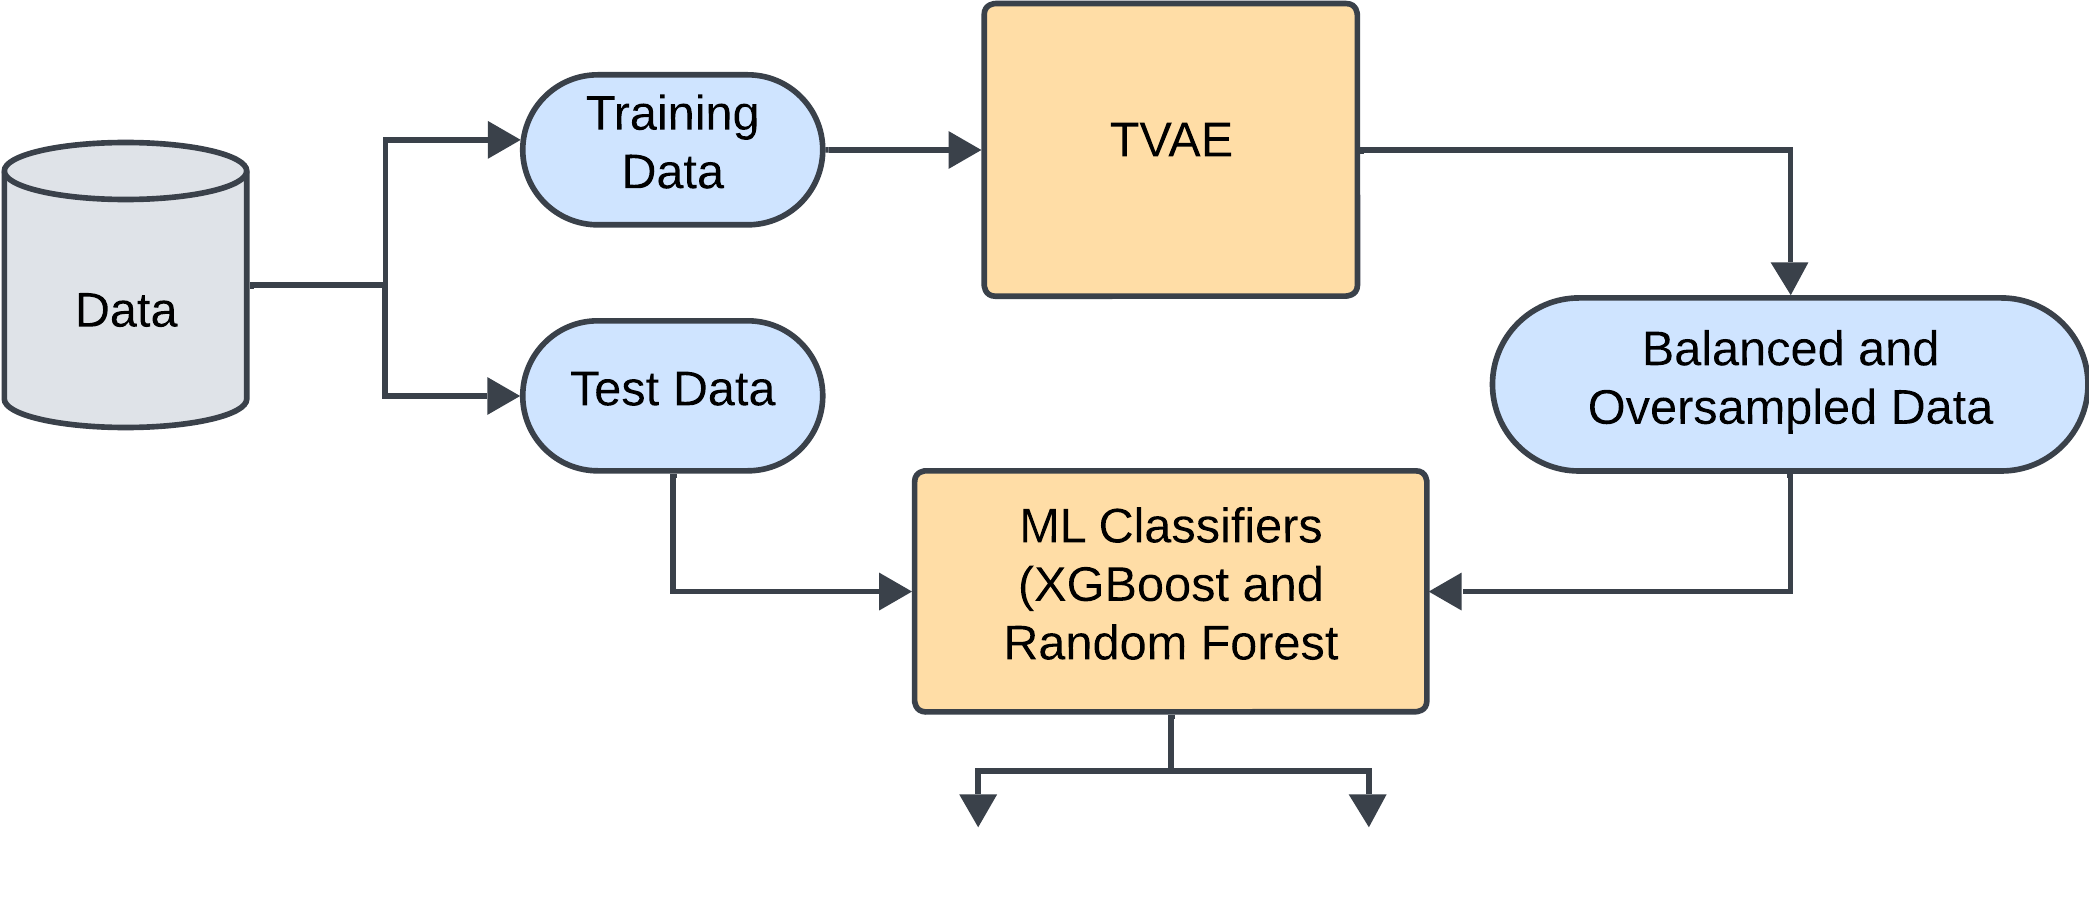
\includegraphics[width=0.85\textwidth]{images/model_tvae.png}
  \caption{Block diagram of the proposed approach to balance the training data and oversample both the classes using synthetic data generated using TVAE}
  \label{fig:model}
\end{figure}

\subsection{Tabular Variational Autoencoder (TVAE)}
TVAE is an adaptation of variational autoencoders that is designed to handle synthetic data generation for tabular data. It was proposed by \cite{XuRp} as a baseline for comparative analysis against their generative model for tabular data, CTGAN. Both the models were designed to deal with the mixed types of data, continuous and discrete, often seen in tabular data. Continuous columns might have a group of values that occur more frequent and discrete or categorical columns may be imbalanced. Moreover, continuous data is usually non-Gaussian making then difficult to be normalized and tabular data usually contains multimodal distributions. 

To deal with the issue of non-Gaussian continuous values TVAE and CTGAN use a \emph{mode-specific} normalization and the discrete columns are \emph{one-hot} encoded. The latent space of the VAE is modified as the joint distribution of \(2N_c + N_d\), where \(N_c\) are the continuous columns and \(N_d\) are discrete columns. For the training and data generation task the continuous columns are assumed to follow a Gaussian distribution and discrete columns follow a categorical PMF. One drawback of TVAE over CTGAN, given in the paper by authors, is the TVAE need to be trained on the actual data whereas CTGAN need not be. 

The specific implementation of TVAE used is the one provided by SDV (Synthetic Data Vault, \citealp{SDV}). SDV is a python library designed for creating synthetic tabular data.

\subsection{Data Preprocessing}
Before the data is fed to the machine learning models it need to be processed into format that can be easily understood and interpreted by the models. The TVAE implementation by SDV does not require any data preprocessing to be done from our side. The model does its own encoding and normalization depending on the type of features. In order to determine the type of features, SDV library requires us to pass the metedata of our data in the form of JSON. As we are using decision tree ensemble models like XGBoost and Random Forest, we do not need to normalize or standardize the data, but we need to encode the features. Therefore, all the nominal features (As mentioned in Table \ref{tab:dataCols}) were one-hot encoded and all the ordinal features were label encoded.

\section{Results and Analysis}  \label{sec:result}
\subsection{Metrics}

\subsection{Evaluation}
We will evaluate our proposed method by comparing the performance of the chosen classification models with different oversampling and undersampling techniques. The proposed approach only applies the oversampling on the training data after splitting the data for test and train, but in order to compare our performance with studies that performed oversampling before the split we have also evaluated additional results by oversampling before the split. The subsection \ref{sec:afterSplit} will discuss the results when the oversampling was performed after the split as mentioned in the proposed approach. The subsection \ref{sec:beforeSplit} will discuss the results when the oversampling was applied before the split.

The TVAE implementation provided by SDV gives the flexibility to tune the model to our requirement through parameters like number of epochs, the encoder dimensions, the decoder dimension, the latent space dimension etc. Therefore, to achieve the best results possible, hyper-parameter tuning was performed by employing Bayesian optimization methods provided by the libraries, \emph{hyperopt} (\citealp{bergstraMakingScienceModel}) and \emph{scikit-optimize}\footnote{https://scikit-optimize.github.io/stable/index.html}. In addition to tuning the TVAE hyper-parameters, the parameters for XGBoost and Random Forest were also tuned, using the same library, for all the oversampling and undersampling methods, using the same search space.

\subsection{Results}
In this section we will look at the evaluation results of our proposed approach. In particular we will look at how the performance of XGBoost and RF are affected by different oversampling and undersampling techniques, and contrast them with the oversampling by using TVAE. The next two subsections will discuss the results with respect to balancing the data after the split and before the split respectively.

\begin{longtable}{|p{1.2cm}|p{1.2cm}|p{2.2cm}|p{2.3cm}|p{2.6cm}|p{2.2cm}|p{2cm}|p{2.2cm}|p{2.6cm}|}
\hline
\textbf{Work} & \textbf{Dataset} & \textbf{Methods} & \textbf{Balance Techniques} & \textbf{Order(Split/Balance)} & \textbf{Result Accuracy} & \textbf{Result Precision} & \textbf{Result Recall} & \textbf{Result F1-score} \\
\hline
[6] & carclaims.txt & ELM & Not Mentioned & Balance the data then split & 74.9\% & 74.9\% & 74.9\% & 74.9\% \\
\hline
[2] & carclaims.txt & Random Forest & SMOTE & Balance the data then split & 94.3\%, 98.6\%, 45.1\% & 94.3\%, 98.6\%, 45.1\% & 94.3\%, 98.6\%, 45.1\% & 94.3\%, 98.6\%, 45.1\%, 61.9\% \\
\hline
[3] & carclaims.txt & Random Forest & SMOTE \newline ROSE & Split Data then balance & 64.3\% \newline 61.34\% & -- \newline 14.1\% & 93.07\% \newline 95.24\% & 23.8\% \newline 22.79\% \\
\hline
[1] & carclaims.txt & Ensemble of SVM, MLP, KNN & FCM (Under Sampling), SMOTE & Balance the data then split & 81.2\% & -- & -- & 94.2\% \\
\hline
[5] & carclaims.txt & 4-layer 1D-CNN & SMOTE \newline CTGAN & Split Data then balance & 81.3\% \newline 79.3\% & 13.6\% \newline 16.7\% & 39.8\% \newline 61.5\% & 20.3\% \newline 26.2\% \\
\hline
Proposed & carclaims.txt & Random Forest XGBoost & TVAE & Split Data then balance and oversample & 87.13\% & 28.66\% & 66.83\% & 87.13\%, 28.66\%, 66.83\%, 40.12\% \\
\hline
\end{longtable}


\subsubsection{Balance data after split} \label{sec:afterSplit}
Figure \ref{fig:xgboost_oversample_after_split} shows the performance metrics for XGBoost, when the balancing of data was done only on the training data after the train-test split is performed. From the figure we can gather that XGBoost was able to achiebe the best F1 score, of 37.1\%, when the data balancing was done using TVAE. Moreover, when the data was augment with additional synthetic samples by TVAE in addition to balancing, the model was able to achieve an F1 score of 40.1\%. The TVAE balanced model was also able to achieve a good recall, indicating that the model is able to identify the fraudulent claims better with TVAE balanced data when compared to other traditional methods like SMOTE, ADASYN or ROS. Data balanced using RUS gives the best recall, but it comes at the cost of precision, meaning that the model is overfitting to the fraudulent cases as an result of under representation of genuine claims due to undersampling.  The data balanced using ROSE achieves the best precision, but performs very poorly in terms of recall, indicating its inability to generalize to the test data. Whereas, the TVAE balanced data is able to achieve very good precision as well, leading to a goof F1 score. Finally in terms of accuracy, the TVAE balanced data achieves an accuracy of 89.1\%, which is very close the best accuracy provided by ROSE.
\begin{figure}
  \centering
  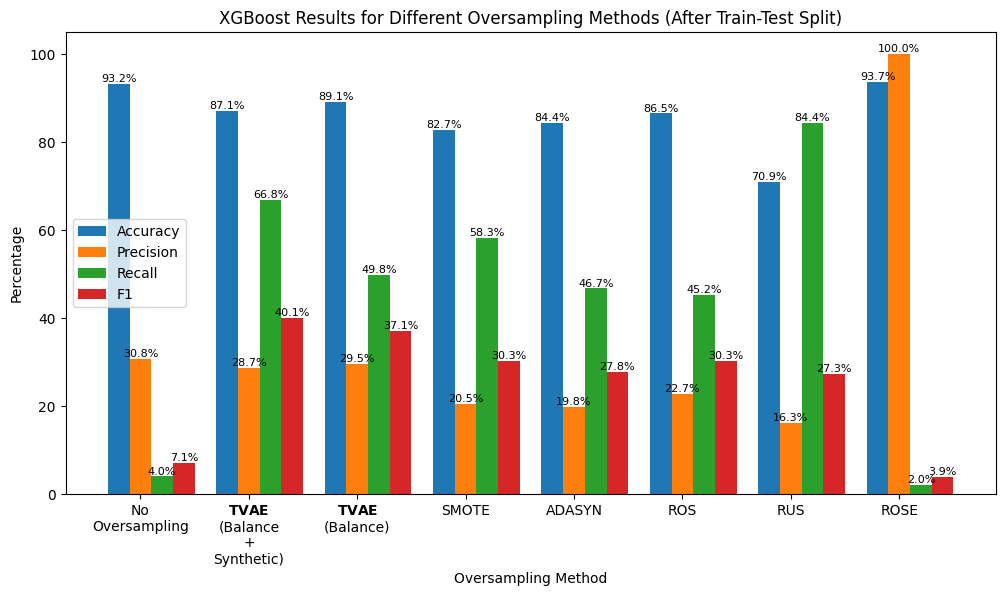
\includegraphics[width=0.85\textwidth]{images/xgboost_oversample_after_split.png}
  \caption{Performance of XGBoost classifier model on data balanced using different techniques after the train-test split}
  \label{fig:xgboost_oversample_after_split}
\end{figure}
Figure \ref{fig:rf_oversample_after_split} shows the performance metrics for RF trained using data balanced after the train-test split. Similar to XGBoost, the TVAE balanced data was able to achieve good F1 score, but was not able to out perform ADASYN and ROS. But in terms of recall, TVAE achieved the best performance next in line to RUS, which as discussed earlier tends to overfit to fraudulent cases leading to low precision. In terms of over all metrics RF seems to perform well with data balanced using ADASYN and ROS.
\begin{figure}
  \centering
  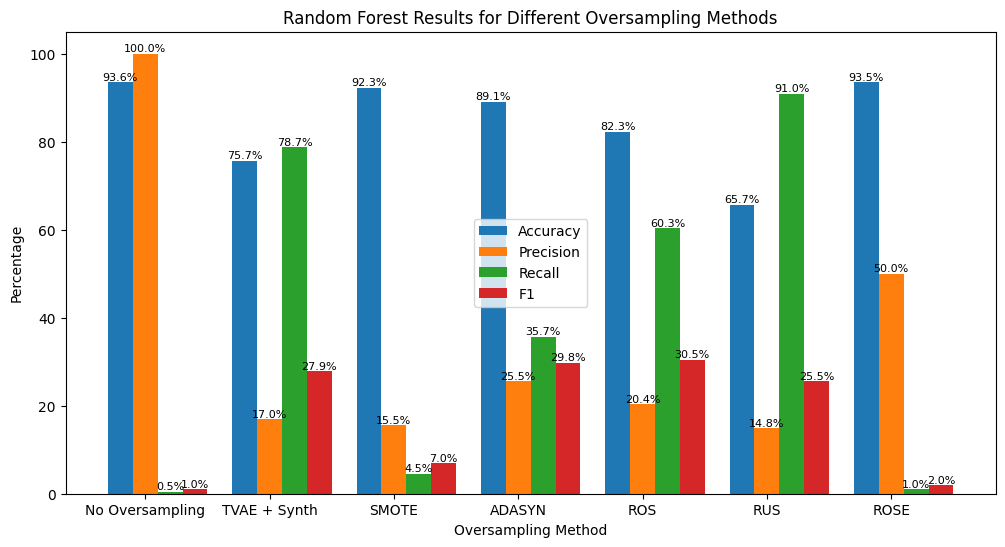
\includegraphics[width=0.85\textwidth]{images/rf_oversample_after_split.png}
  \caption{Performance of Random Forest classifier model on data balanced using different techniques after the train-test split}
  \label{fig:rf_oversample_after_split}
\end{figure}
The overall performance seems to indicate that the models trained on data balanced and augmented using TVAE tend to generalize better to the unseen test data. This might be due the fact that TVAE generates synthetic data using generative approach and distributions, where as traditional approaches, like SMOTE, ADASYN or ROS oversample by creating duplicates of the data.

\subsubsection{Balance data before split} \label{sec:beforeSplit}
Figure \ref{fig:xgboost_oversample_before_split} shows the performance of XGBoost, when it is trained on the data that is first balanced and then split into train and test. At a first glance its obvious that the results for all the balancing techniques are much better compared to previous section. But these results are due to the bias introduced by data leakage. The data balanced, and augmented, using synthetic data generated by TVAE achieved the best accuracy and F1 score in both the cases. The model trained on augmented data performs slightly better compared to the one trained on just balanced data (using TVAE). Following the trend from previous results, RUS has the worst performance due under sampling of genuine cases. Figure \ref{fig:rf_oversample_before_split} shows the performance of RF when its trained on the data that is balanced before the split. It can be seen that the results are very similar to the results with XGBoost.

\begin{figure}
  \centering
  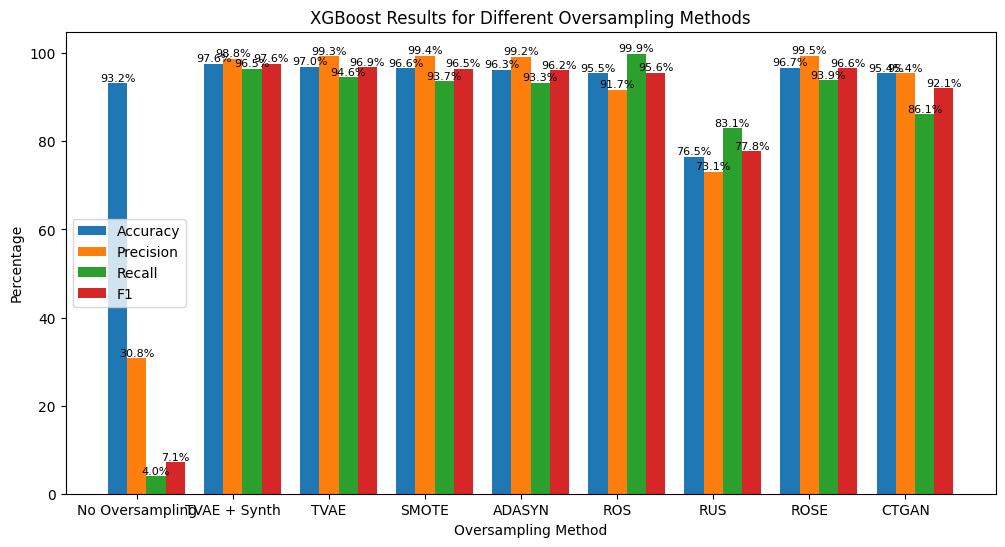
\includegraphics[width=0.85\textwidth]{images/xgboost_oversample_before_split.png}
  \caption{Performance of XGBoost classifier model on data balanced using different techniques before the train-test split}
  \label{fig:xgboost_oversample_before_split}
\end{figure}

\begin{figure}
  \centering
  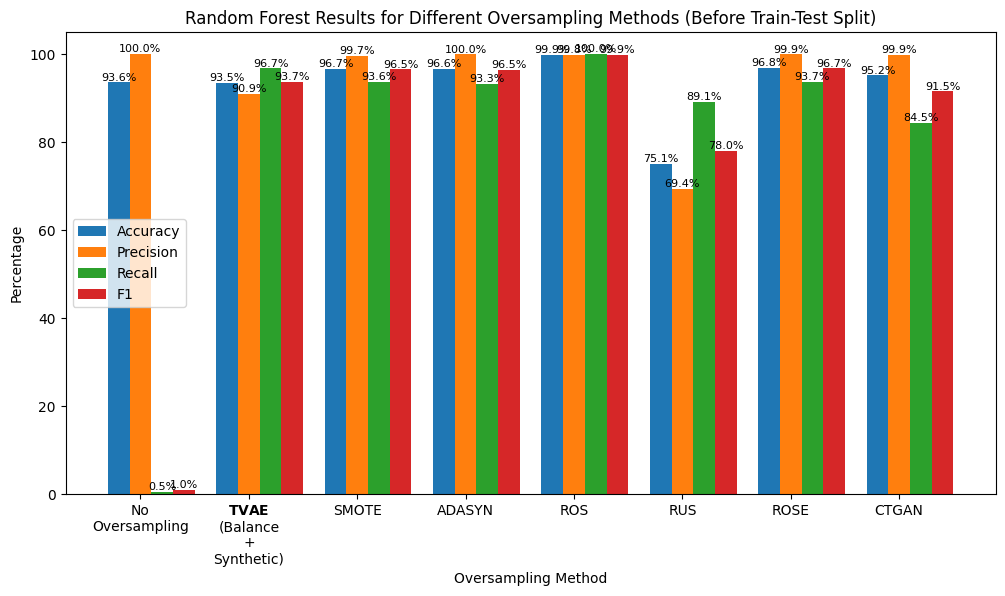
\includegraphics[width=0.85\textwidth]{images/rf_oversample_before_slit.png}
  \caption{Performance of Random Forest classifier model on data balanced using different techniques before the train-test split}
  \label{fig:rf_oversample_before_split}
\end{figure}



\section{Conclusion and Future Work}  \label{sec:conclusion}
To summarize, this project addressed the challenge of severely imbalanced datasets in automobile insurance fraud detection while improving the performance of applied machine learning techniques. A comprehensive review of current balancing methods highlighted persistent challenges, such as handling high-categorical features and generating noisy synthetic data. This study utilized the "carclaims.txt" dataset, which is highly imbalanced and includes 30 categorical features. Preprocessing involved cleaning the data and applying one-hot and label encoding. To address the imbalance issue, TVAE was proposed as a balancing technique that generates realistic synthetic data and effectively handles categorical features. Experimental results demonstrated that TVAE, when combined with Random Forest and XGBoost, achieved the highest F1 score, both before and after splitting, surpassing other balancing techniques (CTGAN, ADAYSN, FCM, SMOTE, ROSE, RUS, and ROS). Furthermore, when more synthetic data generated using TVAE was added to the training data, the model performance improved slightly. These findings underscore the effectiveness of TVAE in mitigating dataset imbalance and improving fraud detection performance. This approach has broader applicability in fields like credit card fraud detection and beyond.
Although we able to outperform existing state-of-the-art performance for the dataset, there is still room for improvement. Future research could explore advanced and broader hyperparameter optimization techniques to further fine-tune the parameters of TVA, XGBoost and Random Forest. Additionally, modern clustering techniques could be leveraged to address the complexity of highly nuanced auto insurance fraud datasets. Incorporating ensemble learning methods may also yield significant improvements in detecting fraudulent claims. These efforts aim to advance the development of more precise and impactful methods for insurance fraud classification. 


\acks{We would like to express our heartfelt gratitude to Dr. Alex Aklson for his guidance and American University of Sharjah for providing access to external GPU resources which significantly speeded up the training process} 

\vskip 0.2in
\bibliography{references}

\end{document}
